\capitulo{7}{Conclusiones y Líneas de trabajo futuras}

%Todo proyecto debe incluir las conclusiones que se derivan de su desarrollo. Éstas pueden ser de diferente índole, dependiendo de la tipología del proyecto, pero normalmente van a estar presentes un conjunto de conclusiones relacionadas con los resultados del proyecto y un conjunto de conclusiones técnicas. 
%Además, resulta muy útil realizar un informe crítico indicando cómo se puede mejorar el proyecto, o cómo se puede continuar trabajando en la línea del proyecto realizado. 
\section{Conclusiones}
Una vez finalizado el proyecto, se considera que se han cumplido todos los requisitos funcionales que se habían declarado en el inicio del mismo. El proyecto ha alcanzado los objetivos propuestos de manera satisfactoria aunque el resultado del modelo predictivo no ha cumplido con las expectativas. Desde un principio se sabía que el conseguir un buen comportamiento del modelo predictivo iba a ser tarea difícil, pues probablemente, el hacer funcionar un modelo de estas características conlleve suficiente dedicación como para un trabajo de final de máster. No obstante, se ha hecho todo lo posible para que el resultado fuese lo más parecido a la realidad. Este proyecto es una buena base desde la que pueden partir futuros desarrollos.

Con todo esto, se ha aprendido a desarrollar una aplicación web que permite la consulta de una predicción de los afloramientos de medusas en las playas de Chile.

Además se han investigado y aplicado diferentes técnicas de \emph{machine learning}, además de realizar un trabajo de tratamiento de datos previo.

Por último, se han aplicado diversos conocimientos aprendidos a lo largo de la carrera tanto de programación como de gestión y diseño del proyecto.

A pesar de esto existen diferentes mejoras que se podrían aplicar en futuras versiones las cuales detallo a continuación:
 
\section{Líneas de trabajo futuras}

A la hora de tratar los datos, nos encontramos que la orografía de la costa cuenta con múltiples golfos y cabos. Esto provoca que no todas las playas tengan orientación hacia el oeste. La información oceánica que se asocia a cada playa, es del cuadrante siguiente a las coordenadas de la misma hacia el oeste, por lo que existen playas cuyos datos no están correctamente asociados. En la figura \ref{tImg} se puede ver un ejemplo. Para corregir este problema se podría implementar un tratamiento de imágenes que devuelva la orientación de la playa para recoger los datos en consecuencia.

\begin{figure}%[!h]
	\centering
	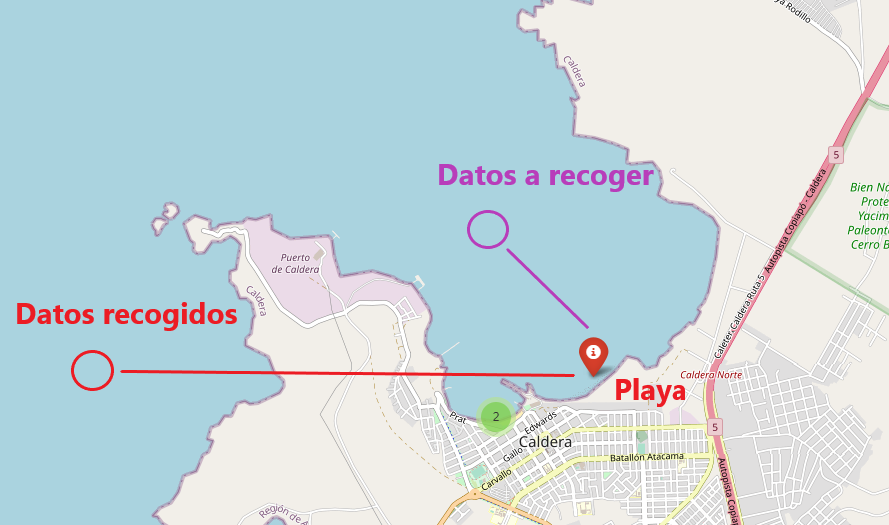
\includegraphics[width=1\textwidth]{lias_futro_playa.png}
	\caption[Tratamiento de imágenes]{Tratamiento de imágenes.}\label{tImg}
\end{figure}


Otro aspecto pendiente sería el tratamiento de los datos como series temporales. Como se indica en el apartado \ref{series_temporales_titutlo}, unicamente se ha utilizado parte de estas técnicas en el entrenamiento del modelo, pero no se han aplicado a la hora del procesamiento previo de los datos.

Por último un aspecto menos relevante, seria la internacionalización de la aplicación. 